\section{Pivotal trees.}

Let $X$ be a metric space.
A point array $(a_1,\dots,a_n)$ in $X$ together with a choice of a graph with $n$ vertexes labeled by  $(a_1,\dots,a_n)$ and a choice of geodesic $[a_i,a_j]$ for every adjacent pair $(a_i,a_j)$ is called \emph{geodesic graph}.

\hide
\begin{wrapfigure}{r}{27 mm}
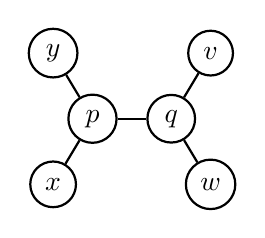
\begin{tikzpicture}[scale=1,
  thick,main node/.style={circle,draw,font=\sffamily\bfseries,minimum size=3mm}]
  \node[main node] (1) at (-1/2,-5/6) {$x$};
  \node[main node] (2) at (0,0){$p$};
  \node[main node] (3) at (-1/2,5/6){$y$};
  \node[main node] (4) at (3/2,5/6) {$v$};
  \node[main node] (5) at (1,0) {$q$};
  \node[main node] (6) at (3/2,-5/6) {$w$};

  \path[every node/.style={font=\sffamily\small}]
   (1) edge node[above]{}(2)
   (2) edge node[above]{}(3)
   (2) edge node[above]{}(5)
   (4) edge node[above]{}(5)
   (5) edge node[above]{}(6);
\end{tikzpicture}
\end{wrapfigure}
\unhide

For geodesic trees we will use the same notation as for labeled combinatoric tree in square brackets; for example $[p,xy(q,vw)]$ will denote the geodesic tree with with combinatorics as on the diagram. 

Fix a geodesic tree $T=[p_1/x_1\dots x_k(p_2/x_{k+1}\dots x_n)]$;
that is, $T$ has two poles $p_1$, $p_2$ and each of the remaining vertexes are adjacent either to $p_1$ or $p_2$ --- the vertexes $x_1,\dots, x_k$ are connected to $p_1$ and $x_{k+1},\dots, x_n$ to $p_2$.

Assume $X$ is a nonnegatively curved Alexandrov space;
in particular the angle is defined for any geodesic hinge. 

A geodesic tree  $\~T=[\~p_1/\~x_1\dots \~x_k(\~p_2/\~x_{k+1}\dots \~x_n)]$ in the Hilbert space $\HH$ will be called \emph{pivotal tree} for $T$
if 
\begin{enumerate}[(i)]
\item $|\~p_1-\~p_2|_\HH= |p_1-p_2|_X$,
\item $|\~p_i-\~x_j|_\HH= |p_i-p_j|_X$ for any edge $[p_i,x_j]$ in $T$ and
\item $\measuredangle[\~p_j\,^{\~x_k}_{\~p_i}]_{\HH}=\measuredangle[\~p_j\,^{\~x_k}_{\~p_i}]_X$
for any hinge  $[p_j\,^{x_k}_{\~p_i}]=([p_j,x_k],[p_j,p_i])$ in $T$.
\end{enumerate}


\begin{thm}{Rigidity lemma}\label{lem:rigidity}
Let $X$ be a nonnegatively curved Alexandrov space and $T=[p_1/x_1\dots x_k(p_2/x_{k+1}\dots x_n)]$ be geodesic tree in $X$
Suppose  $\~T\zz=[\~p_1/\~x_1\dots \~x_k(\~p_2/\~x_{k+1}\dots \~x_n)]$ is a pivotal tree for  $T$.
Assume that
\[|\~x_i-\~x_j|_\HH\le |x_i-x_j|_X 
\eqlbl{eq:pivotal-comparison}\]
for any pair $(i,j)$ and the convex hull $\~K$ of $\{\~x_1,\dots\~x_n\}$ intersects the line thru $\~p_1$ and $\~p_2$.
Then the equality holds in \ref{eq:pivotal-comparison} for each pair $(i,j)$.
\end{thm}

\parit{Proof.}
Let $\~z$ be a point on the line $(\~p_1,\~p_2)$.
Assume that $\~z$ lies on the half-line from $\~p_1$ to $\~p_2$;
otherwise swap the labels of $\~p_1$ and $\~p_2$.

Denote by $\zeta$ the direction of geodesic $[p_1,p_2]$ at $p_1$. 
Set 
\[z=\gexp_{p_1}(|\~z-\~p_1|\cdot \zeta),\]
where $\gexp_{p_1}$ denotes the gradient exponent at $p_1$; see \cite{AKP-book}. 
By comparison, we have
\begin{align*}
|x_i-z|_X &\le |\~x_i-\~z|_{\RR^2}
\end{align*}
for any $i$.

It remains to apply Kirszbraun rigidity theorem (\ref{thm:kirszbraun-rigid}).
\qeds

Recall that $X$ is a nonnegatively curved Alexandrov space.

Assume $[\~p_1/\~x_1\dots \~x_k(\~p_2/\~x_{k+1}\dots \~x_n)]$ is a pivotal tree in $\HH$ for the geodesic tree $[p_1/x_1\dots x_k(p_2/x_{k+1}\dots x_n)]$ in $X$.
Note that by angle comparison, for any $i$ and $j$ we have
\[|\~x_i-\~p_j|_{\HH}\ge |x_i-p_j|_X.\]

It follows that the configuration $\~p_1$, $\~p_2$, $\~x_1,\dots\~x_n\in \HH$ satisfies the tree comparison (see Section~\ref{sec:intro}) if 
\[|\~x_i-\~x_j|_{\HH}\ge |x_i-x_j|_X
\eqlbl{eq:tree-comparison}\]
for all pairs $(i,j)$.

Denote by $\~\xi_i$ the direction of the half-plane containing $\~x_i$ with the boundary line $(\~p_1, \~p_2)$.
The direction $\~\xi_i$ lies in the unit sphere normal to the line $(\~p_1, \~p_2)$;
we may assume that the dimension of the sphere is $n-1$.

Note that up to a motion of $\HH$, a pivotal configuration is completely described by the angles $\measuredangle(\~\xi_i,\~\xi_j)$.
Moreover, the distance $|\~x_i-\~x_j|_\HH$ is determined by $\measuredangle(\~\xi_i,\~\xi_j)$ and the function $\measuredangle(\~\xi_i,\~\xi_j)\mapsto |\~x_i-\~x_j|_\HH$ is nondereasing.

Let us denote by $\alpha_{i,j}$ the minimal angle $\measuredangle(\~\xi_i,\~\xi_j)$ in a pivotal configuration such that \ref{eq:tree-comparison} holds.
Note that the inequality \ref{eq:tree-comparison} is equivalent to
\[\measuredangle(\xi_i,\xi_j)\ge \alpha_{i,j}.\]

\begin{thm}{Corollary}\label{cor:|x-x|}
For any geodesic bipolar tree  in a nonnegatively curved Alexandrov space the following conditions hold:
\begin{enumerate}[(a)]
\item For any pair $i$ and $j$, we have
\[\alpha_{i,j}\le \pi.\]
\item For any triple $i$, $j$ and $k$,  we have
\[\alpha_{i,j}+\alpha_{j,k}+\alpha_{k,i}\le 2\cdot\pi.\]
\end{enumerate}
In other words, if $X$ is a nonnegatively curved Alexandrov space then
\begin{enumerate}[(a)]
\item\label{cor:|x-x|:a} For any broken geodesic line $[p_1/x_1(p_2/x_2)]$ in  $X$ there is a pivotal tree $[\~p_1/\~x_1(\~p_2/\~x_2)]$ such that 
\[|\~x_1-\~x_2|_{\HH}\ge |x_1-x_2|_X.\]

\item\label{cor:|x-x|:b} For any $[p_1/x_1x_2(p_2/x_3)]$ in $X$, there is a pivotal tree $[\~p_1/\~x_1\~x_2(\~p_2/\~x_3)]$ such that 
\begin{align*}
|\~x_i-\~x_j|_{\HH}&\ge |x_i-x_j|_X.
\end{align*}
for all $i$ and $j$.
\end{enumerate}

\hide
\begin{center}
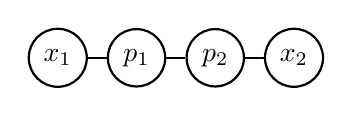
\begin{tikzpicture}[scale=1,
  thick,main node/.style={circle,draw,font=\sffamily\bfseries,minimum size=3mm}]
  \node[main node] (2) at (1,0){$p_1$};
  \node[main node] (3) at (0,0){$x_1$};
  \node[main node] (4) at (3,0) {$x_2$};
  \node[main node] (5) at (2,0) {$p_2$};
  \path[every node/.style={font=\sffamily\small}]
   (2) edge node[above]{}(3)
   (2) edge node[above]{}(5)
   (4) edge node[above]{}(5);
\end{tikzpicture}
\hskip10mm
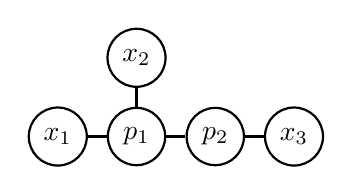
\begin{tikzpicture}[scale=1,
  thick,main node/.style={circle,draw,font=\sffamily\bfseries,minimum size=3mm}]
  \node[main node] (1) at (0,0) {$x_1$};
  \node[main node] (2) at (1,0){$p_1$};
  \node[main node] (3) at (1,1){$x_2$};
  \node[main node] (4) at (3,0) {$x_3$};
  \node[main node] (5) at (2,0) {$p_2$};
  

  \path[every node/.style={font=\sffamily\small}]
   (1) edge node[above]{}(2)
   (2) edge node[above]{}(3)
   (2) edge node[above]{}(5)
   (4) edge node[above]{}(5);
\end{tikzpicture}
\end{center}
\unhide

\end{thm}

\parit{Proof; (\ref{cor:|x-x|:a}).}
Consider the pivotal tree $[\~p_1/\~x_1(\~p_2/\~x_2)]$ (which is a polygonal path) with $\measuredangle(\~\xi_1,\~\xi_2)=\pi$.
Note that the points $\~p_1,\~x_1,\~p_2,\~x_2$ are coplanar and the points $\~x_1$ and $\~x_2$ lie on the opposite sides from the line $(\~p_1,\~p_2)$.
It remains to apply the rigidity lemma.

\parit{(\ref{cor:|x-x|:b}).} By \textit{(\ref{cor:|x-x|:a})}, we can assume that \[\alpha_{1,3}+\alpha_{2,3}>\pi.
\eqlbl{sum>pi}\]

Consider the pivotal tree $[\~p_1/\~x_1\~x_2(\~p_2/\~x_3)]$ which lies in a 3-dimesional subspace in such a way that the points $\~x_1$ and $\~x_2$ lie on the opposite sides from the plane containing $\~p_1,\~p_2,\~x_3$, and 
\begin{align*}
\measuredangle(\~\xi_1,\~\xi_3)&=\alpha_{1,3},
&
\measuredangle(\~\xi_2,\~\xi_3)&=\alpha_{2,3}.
\end{align*}
By \ref{sum>pi}, the convex hull $\~K$ of $\{\~x_1,\~x_2,\~x_3\}$ intersects the line $(\~p_1,\~p_2)$.
It remains to apply the rigidity lemma.
\qeds

Note that \textit{(\ref{cor:|x-x|:a})} and \textit{(\ref{cor:|x-x|:b})} implies that nonnegatively curved Alexandrov space satisfies 1(1)-tree and 2(1)-tree comparisons. 
However, 1(1)-tree comparison follows directly from the triangle inequality.



\section{2(2)-tree and 3(1)-tree comparisons}\label{6-dipole}

The following theorem generalizes Theorem \ref{thm:3(1)+2(2)}.
It says in particular, that the comparisons for the following two trees holds in nonnegatively Alexandrov spaces.

\hide
\begin{center}
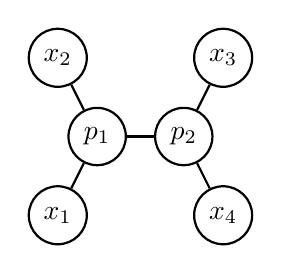
\begin{tikzpicture}[scale=1,
  thick,main node/.style={circle,draw,font=\sffamily\bfseries,minimum size=3mm}]

  \node[main node] (1) at (-1/2,0) {$x_1$};
  \node[main node] (2) at (0,1){$p_1$};
  \node[main node] (3) at (-1/2,2){$x_2$};
  \node[main node] (4) at (3/2+.1,0) {$x_4$};
  \node[main node] (5) at (1.1,1) {$p_2$};
  \node[main node] (6) at (3/2+.1,2) {$x_3$};

  \path[every node/.style={font=\sffamily\small}]
   (1) edge node[above]{}(2)
   (2) edge node[above]{}(3)
   (2) edge node[above]{}(5)
   (4) edge node[above]{}(5)
   (5) edge node[above]{}(6);
\end{tikzpicture}
\hskip10mm
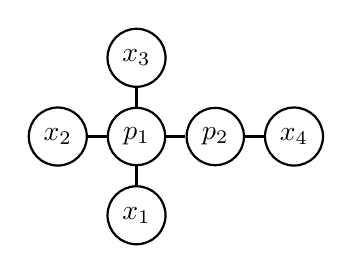
\begin{tikzpicture}[scale=1,
  thick,main node/.style={circle,draw,font=\sffamily\bfseries,minimum size=3mm}]

  \node[main node] (1) at (0,0) {$x_1$};
  \node[main node] (2) at (0,1){$p_1$};
  \node[main node] (3) at (-1,1){$x_2$};
  \node[main node] (4) at (2,1) {$x_4$};
  \node[main node] (5) at (1,1) {$p_2$};
  \node[main node] (6) at (0,2) {$x_3$};

  \path[every node/.style={font=\sffamily\small}]
   (1) edge node[above]{}(2)
   (2) edge node[above]{}(3)
   (2) edge node[above]{}(5)
   (2) edge node[above]{}(6)
   (4) edge node[above]{}(5);
\end{tikzpicture}
\end{center}
\unhide


\begin{thm}{Theorem}\label{2(2)+3(1)}
Let $X$ be an nonnegatively curved Alexandrov space.
Then for any geodesic 2(2)-tree (or 3(1)-tree) there is a pivotal tree satisfying the corresponding tree comparison.


In particular, any nonnegatively curved Alexandrov space satisfies the 2(2)-tree comparison as well as 3(1)-tree comparison.

\end{thm}

The proofs in the two cases are nearly identical; they differ only by the choice made in the first line.

\parit{Proof.} 
Fix a geodesic tree $[p_1/x_1x_2(p_2/x_3x_4)]$ or $[p_1/x_1x_2x_3(p_2/x_4)]$.
Define the values $\{\alpha_{i,j}\}$ for each pair $i,j$ as in the previous section.

Recall that $p_1$ and $p_2$ are the poles of the tree and each of remaining vertexes $x_1,x_2, x_3,x_4$ are connected to one of the poles.


Fix a smooth monotonic function $\phi\:\RR\to\RR$ such that $\phi(x)=0$ if $x\ge 0$ and $\phi(x)>0$ if $x<0$.
Consider a configuration of 4 points $\~\xi_1,\~\xi_2,\~\xi_3,\~\xi_4$ in $\SS^3$ which minimize the \emph{energy}
\[E(\~\xi_1,\~\xi_2,\~\xi_3,\~\xi_4)
=
\sum_{i<j}\phi(\measuredangle(\~\xi_i,\~\xi_j)-\alpha_{i,j}).\]

Consider the geodesic graph $\Gamma$ with 4 vertexes $\~\xi_1,\~\xi_2,\~\xi_3,\~\xi_4$ in $\SS^3$, where 
$\~\xi_i$ is adjacent to $\~\xi_j$ if $\measuredangle(\~\xi_i,\~\xi_j)<\alpha_{i,j}$.
If the comparison does not hold then $\Gamma$ is not empty.

Note that a vertex of $\Gamma$ can not lie in an open hemisphere with all its adjacent vertexes. 
Indeed, if it would be the case then we could move this vertex increasing the distances to all its adjacent vertexes.
Along this move the energy decreases which is not possible.

Note that by Corollary \ref{cor:|x-x|}, degree of any vertex is at least 2.
Indeed existence of a vertex of degree 1 contradicts \ref{cor:|x-x|}\textit{\ref{cor:|x-x|:a}} and existence of a vertex of degree 0 contradicts \ref{cor:|x-x|}\textit{\ref{cor:|x-x|:b}}.

Therefore the graph $\Gamma$ is isomorphic to one the following three graphs.

\hide
\begin{center}
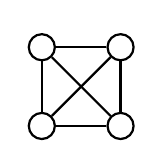
\begin{tikzpicture}[scale=1,
  thick,main node/.style={circle,draw,font=\sffamily\bfseries,minimum size=3mm}]

  \node[main node] (1) at (0,0) {};
  \node[main node] (2) at (0,1){};
  \node[main node] (3) at (1,1){};
  \node[main node] (4) at (1,0) {};

  \path[every node/.style={font=\sffamily\small}]
   (1) edge node[above]{}(2)
   (2) edge node[above]{}(3)
   (2) edge node[above]{}(4)
   (3) edge node[above]{}(1)
   (3) edge node[above]{}(4)
   (1) edge node[above]{}(4);
\end{tikzpicture}
\hskip20mm
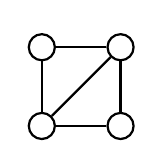
\begin{tikzpicture}[scale=1,
  thick,main node/.style={circle,draw,font=\sffamily\bfseries,minimum size=3mm}]

  \node[main node] (1) at (0,0) {};
  \node[main node] (2) at (0,1){};
  \node[main node] (3) at (1,1){};
  \node[main node] (4) at (1,0) {};

  \path[every node/.style={font=\sffamily\small}]
   (1) edge node[above]{}(2)
   (2) edge node[above]{}(3)
   (3) edge node[above]{}(1)
   (3) edge node[above]{}(4)
   (1) edge node[above]{}(4);
\end{tikzpicture}
\hskip20mm
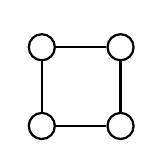
\begin{tikzpicture}[scale=1,
  thick,main node/.style={circle,draw,font=\sffamily\bfseries,minimum size=3mm}]

  \node[main node] (1) at (0,0) {};
  \node[main node] (2) at (0,1){};
  \node[main node] (3) at (1,1){};
  \node[main node] (4) at (1,0) {};

  \path[every node/.style={font=\sffamily\small}]
   (1) edge node[above]{}(2)
   (2) edge node[above]{}(3)
   (3) edge node[above]{}(4)
   (1) edge node[above]{}(4);
\end{tikzpicture}
\end{center}
\unhide

The 6-edege case (that is, the complete graph with 4 vertexes) can not appear by the rigidity lemma (see \ref{lem:rigidity}).

To do the remaining two cases, note that since the energy is minimal, the angle between the edges at every vertex of degree 2 of $\Gamma$ has to be $\pi$. 
That is, the pair of edges at such vertex forms a geodesic.

Consider the 5-edge graph on the diagram.
By the observation above the both triangles in the graph run along one equator.
The latter contradicts Corollary \ref{cor:|x-x|}\textit{\ref{cor:|x-x|:b}}.

For the 4-edge graph (that is, for 4-cycle)
by the same observation we have 4 points lie on the equator; 
moving the even pair to the north pole and odd pair to the south pole will decrease the energy, a contradiction.
\qeds
